% chapters/dcripple.tex
% generated from dclink_2w_ripple_phase.tex
\chapter{Phase relationship of the DC-link ripple at twice the line frequency}
\label{ch:dcripple}
\begin{chapabstract}
This note derives the exact relation between the phase of the AC-side quantities
of a single-phase converter, oscillating at the line angular frequency $\omega$,
and the phase of the resulting DC-link voltage ripple at $2\omega$. The
double-line-frequency ripple is shown to be the time integral of the pulsating
component of the instantaneous port power, so that its $2\omega$ phasor
\emph{leads} the pulsating-power phasor by exactly $\SI{90}{\degree}$, and its
peak occurs at the line electrical angle $\theta = \varphi/2 - \SI{45}{\degree}$,
where $\varphi$ is the displacement angle between line voltage and line current.
Capacitor ESR, DC-side impedance and control-loop effects are then discussed,
together with the consequences for DC-link ripple compensation, feed-forward
duty-cycle correction and active power decoupling.
\end{chapabstract}

\section{Scope and conventions}

Consider a single-phase full bridge connected to an AC line through an inductive
or LCL filter, and to a DC link consisting of a capacitance $C$ in parallel with
a DC source and/or a DC load (the topology is described here verbally:
DC source $\rightarrow$ $C$ $\rightarrow$ H-bridge $\rightarrow$ filter
$\rightarrow$ AC line).

The following conventions are used throughout:

\begin{itemize}
  \item the AC quantities are referred to the \emph{point of connection} of the
        converter, downstream of the filter, so that the port power is the power
        actually exchanged with the line;
  \item power is counted positive when it flows \emph{from the DC link to the AC
        side} (inverter operation). Rectifier / active-front-end operation is
        obtained by $\varphi \rightarrow \varphi + \pi$, i.e.\ by a sign
        reversal of $P$ and $Q$;
  \item the line voltage is taken as the phase reference,
        \begin{equation}
          v(t) = \hat V \cos(\omega t) = \hat V \cos \theta ,
          \qquad \theta \triangleq \omega t ;
        \end{equation}
  \item the line current lags the voltage by the displacement angle $\varphi$,
        \begin{equation}
          i(t) = \hat I \cos(\omega t - \varphi) .
        \end{equation}
\end{itemize}

Switching-frequency components are neglected: only the low-frequency (baseband)
behaviour is of interest here.

\section{Instantaneous power of a single-phase port}

The instantaneous power exchanged with the line is
\begin{equation}
  p(t) = v(t)\, i(t)
       = \hat V \hat I \cos(\omega t)\cos(\omega t - \varphi)
       = \frac{\hat V \hat I}{2}\Bigl[\cos\varphi + \cos(2\omega t - \varphi)\Bigr].
\end{equation}

Introducing the RMS quantities $V=\hat V/\sqrt 2$, $I=\hat I/\sqrt 2$ and
\begin{equation}
  P = VI\cos\varphi, \qquad
  Q = VI\sin\varphi, \qquad
  S = VI = \sqrt{P^2+Q^2},
\end{equation}
this becomes
\begin{equation}
  \boxed{\;
  p(t) = \underbrace{P}_{\text{mean}}
       + \underbrace{S\cos(2\omega t - \varphi)}_{\tilde p(t)} \;}
  \label{dcripple:eq:p}
\end{equation}
or, in the equivalent grid-referenced form obtained by expanding the cosine,
\begin{equation}
  p(t) = P\bigl(1 + \cos 2\omega t\bigr) + Q \sin 2\omega t .
  \label{dcripple:eq:pPQ}
\end{equation}

Equation~\eqref{dcripple:eq:pPQ} is the form to be preferred for implementation, because
$P$ and $Q$ are directly available in any grid-connected control structure
(DQ or PQ estimator, or the outputs of the outer loops), while $\varphi$ is not.

Two facts follow immediately and are worth stating explicitly:
\begin{enumerate}
  \item the amplitude of the pulsating power is the \emph{apparent} power $S$,
        not the active power: a converter operating at zero power factor still
        produces full-amplitude $2\omega$ ripple;
  \item the phase of $\tilde p$ with respect to the doubled line angle $2\theta$
        is $-\varphi$: reactive power \emph{rotates} the pulsating power, it does
        not attenuate it.
\end{enumerate}

\section{DC-link energy balance and voltage ripple}

Assume for the moment an ideal DC source delivering the constant power $P$, an
ideal (lossless, zero-ESR) capacitor $C$, and a lossless bridge. The
instantaneous mismatch between the constant power supplied by the source and the
pulsating power absorbed by the AC port must be provided by the capacitor:
\begin{equation}
  \frac{\mathrm d}{\mathrm d t}\left(\frac{1}{2}C v_{\mathrm{dc}}^2(t)\right)
  = P - p(t) = -\tilde p(t) = -S\cos(2\omega t - \varphi).
  \label{dcripple:eq:energy}
\end{equation}

Integrating,
\begin{equation}
  \frac{1}{2}C v_{\mathrm{dc}}^2(t)
  = \frac{1}{2}C V_{\mathrm{dc}}^2
    - \frac{S}{2\omega}\sin(2\omega t - \varphi),
  \label{dcripple:eq:w}
\end{equation}
where $V_{\mathrm{dc}}$ is the DC (mean-square) value of the link voltage. Hence
the \emph{exact} large-signal solution
\begin{equation}
  v_{\mathrm{dc}}(t)
  = V_{\mathrm{dc}}\sqrt{\,1 - \frac{S}{\omega C V_{\mathrm{dc}}^2}
    \sin(2\omega t - \varphi)\,}.
  \label{dcripple:eq:exact}
\end{equation}

The peak-to-peak energy swing of the capacitor is
\begin{equation}
  \Delta W_{\mathrm{pp}} = \frac{S}{\omega},
  \label{dcripple:eq:dW}
\end{equation}
which is the quantity that fixes the minimum storage requirement of any passive
or active solution and is independent of the chosen DC voltage.

\subsection{Small-ripple linearisation}

For $\Delta v_{\mathrm{dc}} \ll V_{\mathrm{dc}}$ (the normal design case, ripple
of a few percent), a first-order expansion of \eqref{dcripple:eq:exact} gives
\begin{equation}
  \boxed{\;
  \Delta v_{\mathrm{dc}}(t) \simeq
  -\,\frac{S}{2\omega C V_{\mathrm{dc}}}\,\sin(2\omega t - \varphi)
  = \hat V_r \cos\!\left(2\omega t - \varphi + \frac{\pi}{2}\right),
  \qquad
  \hat V_r = \frac{S}{2\omega C V_{\mathrm{dc}}} \;}
  \label{dcripple:eq:ripple}
\end{equation}
or, in the $P$--$Q$ form,
\begin{equation}
  \Delta v_{\mathrm{dc}}(t) \simeq
  -\,\frac{1}{2\omega C V_{\mathrm{dc}}}
    \Bigl(P \sin 2\omega t - Q \cos 2\omega t\Bigr).
  \label{dcripple:eq:ripplePQ}
\end{equation}

The second-order term neglected in \eqref{dcripple:eq:ripple} generates a small
$4\omega$ component of relative amplitude $\hat V_r/(4V_{\mathrm{dc}})$ with
respect to the $2\omega$ one; for a \SI{5}{\percent} ripple this is about
\SI{1.25}{\percent} of the $2\omega$ ripple and is normally negligible, but it
is the reason why a purely sinusoidal $2\omega$ cancellation never gives exactly
zero residual ripple.

\section{The phase relation}

\subsection{Statement of the result}

A phase difference between a quantity at $\omega$ and a quantity at $2\omega$ is
not defined in the usual phasor sense: the two rotate at different speeds. The
relation is well posed only if both are expressed as functions of the same
angular variable, i.e.\ of the line electrical angle $\theta = \omega t$ measured
from a common time origin (in practice, the output of the PLL). With that
convention the results above give
\begin{equation}
  \tilde p(\theta) = S \cos(2\theta - \varphi),
  \qquad
  \Delta v_{\mathrm{dc}}(\theta) =
  \hat V_r \cos\!\left(2\theta - \varphi + \frac{\pi}{2}\right).
  \label{dcripple:eq:theta}
\end{equation}

Three equivalent statements of the same result:

\begin{description}
  \item[In the $2\omega$ domain.] Treating $2\omega$ quantities as phasors, the
        DC-link ripple \emph{leads} the pulsating power by exactly
        \SI{90}{\degree}:
        \begin{equation}
          \Delta \bar V_{\mathrm{dc}} =
          \frac{1}{\mathrm{j}\,2\omega\,C\,V_{\mathrm{dc}}}\,
          \bigl(-\tilde{\bar P}\bigr)
          \;\Longrightarrow\;
          \angle \Delta \bar V_{\mathrm{dc}}
          = \angle \tilde{\bar P} + \frac{\pi}{2}.
        \end{equation}
        The \SI{90}{\degree} lead is the composition of the
        $-\SI{90}{\degree}$ of the integration in \eqref{dcripple:eq:energy} with the
        $\SI{180}{\degree}$ of the minus sign (the capacitor discharges when the
        AC side demands more than the average).
  \item[Relative to the line voltage.] The ripple maxima occur at the line
        angles
        \begin{equation}
          \boxed{\;\theta_{\max} = \frac{\varphi}{2} - \SI{45}{\degree}
          \pmod{\SI{180}{\degree}} \;}
          \label{dcripple:eq:thmax}
        \end{equation}
        and the minima \SI{90}{\degree} later. Note the factor $1/2$: a change
        $\Delta\varphi$ of the displacement angle shifts the ripple by
        $\Delta\varphi/2$ in line angle (i.e.\ by $\Delta\varphi$ in the doubled
        angle).
  \item[Relative to the line current.] Since the current peaks at
        $\theta = \varphi$, the ripple peak occurs at
        $\theta_{\max} - \varphi = -\varphi/2 - \SI{45}{\degree}$ with respect
        to the current peak.
\end{description}

\subsection{Special cases and sanity checks}

Table~\ref{dcripple:tab:cases} collects the position of the DC-link voltage maximum for
some relevant operating points, with the inverter sign convention
($p > 0$ from DC to AC).

\begin{table}[htbp]
  \centering
  \caption{Position of the DC-link voltage ripple peak, referred to the positive
  peak of the line voltage, for different displacement angles.}
  \label{dcripple:tab:cases}
  \begin{tabular}{lccl}
    \toprule
    Operating point & $\varphi$ & $\theta_{\max}$ & Remark \\
    \midrule
    Unity PF, inverting        & \SI{0}{\degree}   & \SI{-45}{\degree}
      & ripple peak \SI{45}{\degree} \emph{before} the voltage peak \\
    PF $=0.866$ lagging        & \SI{30}{\degree}  & \SI{-30}{\degree} & \\
    Pure inductive $Q$ ($Q>0$) & \SI{90}{\degree}  & \SI{0}{\degree}
      & ripple peak \emph{at} the voltage peak, $P=0$ \\
    Unity PF, rectifying (AFE) & \SI{180}{\degree} & \SI{+45}{\degree}
      & mirror image of the inverting case \\
    Pure capacitive $Q$ ($Q<0$)& \SI{-90}{\degree} & \SI{-90}{\degree}
      & ripple peak at the voltage zero crossing \\
    \bottomrule
  \end{tabular}
\end{table}

The unity-power-factor case deserves a comment because it is the one most often
misremembered. At $\varphi=0$ the instantaneous power is maximum at the voltage
peak, so one is tempted to expect the DC-link voltage to be maximum or minimum
there. It is neither: at $\theta = 0$ the capacitor is at its \emph{nominal}
value and is discharging at maximum rate, because the ripple is the
\emph{integral} of the power mismatch, not the mismatch itself. The extremes
occur at the zeros of $\tilde p$, i.e.\ \SI{45}{\degree} away from the voltage
peaks and zero crossings.

\subsection{Waveforms}

Figure~\ref{dcripple:fig:wave} shows the normalised waveforms for $\varphi=0$: line
voltage, line current, instantaneous power and DC-link ripple.

\begin{figure}[htbp]
  \centering
  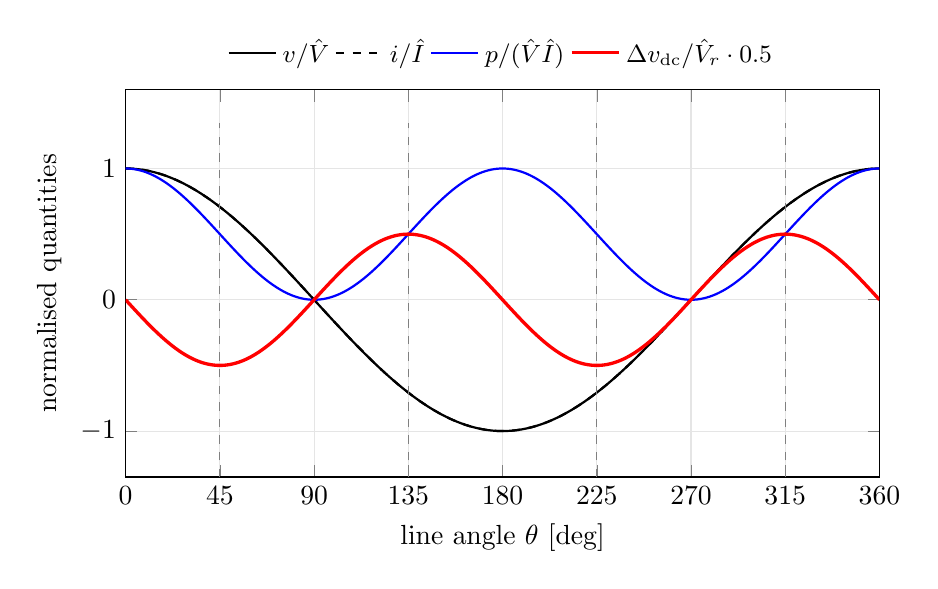
\begin{tikzpicture}
    \begin{axis}[
      width=0.92\textwidth, height=6.5cm,
      xlabel={line angle $\theta$ [deg]},
      ylabel={normalised quantities},
      xmin=0, xmax=360, xtick={0,45,90,135,180,225,270,315,360},
      ymin=-1.35, ymax=1.6,
      grid=both, grid style={gray!20},
      legend columns=4, legend style={at={(0.5,1.03)}, anchor=south,
                                      draw=none, fill=none, font=\small},
      domain=0:360, samples=361,
      ]
      \addplot[thick, black] {cos(x)};
      \addlegendentry{$v/\hat V$}
      \addplot[thick, black, dashed] {cos(x)};
      \addlegendentry{$i/\hat I$}
      \addplot[thick, blue] {0.5*(1+cos(2*x))};
      \addlegendentry{$p/(\hat V\hat I)$}
      \addplot[very thick, red] {-0.5*sin(2*x)};
      \addlegendentry{$\Delta v_{\mathrm{dc}}/\hat V_r \cdot 0.5$}
      \draw[gray, dashed] (axis cs:45,-1.35) -- (axis cs:45,1.35);
      \draw[gray, dashed] (axis cs:135,-1.35) -- (axis cs:135,1.35);
      \draw[gray, dashed] (axis cs:225,-1.35) -- (axis cs:225,1.35);
      \draw[gray, dashed] (axis cs:315,-1.35) -- (axis cs:315,1.35);
    \end{axis}
  \end{tikzpicture}
  \caption{Normalised waveforms for $\varphi=0$ (unity power factor). The
  vertical dashed lines mark the extremes of the DC-link ripple, located
  \SI{45}{\degree} away from the peaks and the zero crossings of the line
  voltage. For clarity the ripple is drawn with half amplitude and with the
  inverter sign convention: at $\theta=\SI{135}{\degree}$ the capacitor is at
  its maximum, i.e.\ it has been charging while $p < P$.}
  \label{dcripple:fig:wave}
\end{figure}

\section{Non-idealities that modify the phase}

\subsection{Capacitor ESR}

The current flowing in the DC-link capacitor is, to first order,
\begin{equation}
  i_C(t) = \frac{-\tilde p(t)}{v_{\mathrm{dc}}(t)}
         \simeq -\frac{S}{V_{\mathrm{dc}}}\cos(2\omega t - \varphi),
\end{equation}
so the ESR contribution $R_{\mathrm{esr}} i_C$ is in phase opposition with
$\tilde p$, while the capacitive contribution leads it by \SI{90}{\degree}.
Their sum gives an additional phase lead
\begin{equation}
  \Delta\psi_{\mathrm{esr}} = \arctan\!\bigl(2\omega C R_{\mathrm{esr}}\bigr)
  = \arctan\!\left(\tan\delta\right)_{@2\omega},
\end{equation}
i.e.\ exactly the loss angle of the capacitor evaluated at $2\omega$, and an
amplitude increase by the factor $\sqrt{1+(2\omega C R_{\mathrm{esr}})^2}$. For
a film capacitor bank at \SI{100}{\hertz} or, worse, at \SI{33.4}{\hertz}, this
correction is well below \SI{1}{\degree} and can be ignored; for large
electrolytic banks it can reach a few degrees and, more importantly, is the
dominant loss mechanism.

\subsection{Finite DC-source and load impedance}

Equation~\eqref{dcripple:eq:energy} assumes that the DC side is a constant-power port at
$2\omega$. In reality the DC source (or the load, e.g.\ a machine-side inverter)
presents a finite impedance and absorbs part of the $2\omega$ current. If
$Z_{\mathrm{dc}}(\mathrm j 2\omega)$ is the equivalent DC-side impedance seen in
parallel with $C$, the ripple becomes
\begin{equation}
  \Delta \bar V_{\mathrm{dc}} =
  \frac{-\tilde{\bar P}}{V_{\mathrm{dc}}}\cdot
  \frac{Z_{\mathrm{dc}} \,\|\, \bigl(1/\mathrm j 2\omega C\bigr)}{1},
\end{equation}
which reduces to \eqref{dcripple:eq:ripple} for $|Z_{\mathrm{dc}}| \gg 1/(2\omega C)$.
A machine-side inverter operating with a fast torque loop behaves as a constant
power load, i.e.\ as a \emph{negative} resistance at low frequency, which
increases the ripple and rotates its phase; this coupling must be checked when
the two converters share the same link.

\subsection{Voltage-loop reaction}

If the outer DC-link voltage regulator has appreciable gain at $2\omega$, it
modulates the active current reference at $2\omega$, which reacts back on
$\tilde p$ and hence on the ripple itself. The result is both a change of
amplitude and a phase rotation of the ripple, and, on the AC side, a third
harmonic of the line current. This is the standard reason for placing a notch at
$2\omega$ in the voltage loop, or for using $v_{\mathrm{dc}}^2$ (i.e.\ the
energy) as controlled variable, which also linearises \eqref{dcripple:eq:energy} exactly.

\section{Consequences for DC-link compensation}

\subsection{Third harmonic generated by the uncompensated ripple}

If the modulator uses a fixed nominal value $V_{\mathrm{dc}}$ instead of the
measured link voltage, the duty ratio is $d(t)=v^{*}(t)/V_{\mathrm{dc}}$ and the
bridge produces
\begin{align}
  v_{\mathrm{out}}(t) &= d(t)\,v_{\mathrm{dc}}(t)
   = \frac{\hat V \cos\theta}{V_{\mathrm{dc}}}
     \Bigl[V_{\mathrm{dc}} + \hat V_r\cos(2\theta+\psi)\Bigr] \notag \\
   &= \hat V\cos\theta
    + \frac{\hat V \delta}{2}\cos(\theta+\psi)
    + \frac{\hat V \delta}{2}\cos(3\theta+\psi),
    \qquad
    \delta \triangleq \frac{\hat V_r}{V_{\mathrm{dc}}},
    \quad \psi = \frac{\pi}{2}-\varphi .
  \label{dcripple:eq:third}
\end{align}

Two effects appear:
\begin{itemize}
  \item a \textbf{third harmonic} of relative amplitude $\delta/2$: a
        \SI{5}{\percent} peak ripple produces \SI{2.5}{\percent} of third
        harmonic voltage, which the filter impedance converts into a current
        harmonic that is generally not acceptable against IEEE~519 or EN~50160
        limits;
  \item a \textbf{fundamental perturbation} of the same amplitude $\delta/2$ and
        phase $\psi$, which at unity power factor ($\psi = \SI{90}{\degree}$) is
        in quadrature with the reference and therefore appears to the current
        loop as a spurious reactive component.
\end{itemize}

The cure is trivial and should always be implemented: divide the voltage
reference by the \emph{instantaneous measured} link voltage,
$d(t)=v^{*}(t)/v_{\mathrm{dc}}(t)$, with an adequate measurement bandwidth
(at least a decade above $2\omega$) and taking care of the sampling instant, so
that the $2\omega$ content is reconstructed and not aliased.

\subsection{Feed-forward reference for an active decoupling stage}

An active power decoupling (APD) circuit must absorb $\tilde p$ in
\eqref{dcripple:eq:p}. Its power reference can be built directly from the measured
active and reactive power using \eqref{dcripple:eq:pPQ},
\begin{equation}
  p^{*}_{\mathrm{apd}}(t) = \hat P \cos 2\theta + \hat Q \sin 2\theta ,
\end{equation}
where $\hat P$ and $\hat Q$ are slow (filtered) estimates and $\theta$ comes
from the PLL. Equivalently, in energy form, the storage element of the APD must
track
\begin{equation}
  \tilde w^{*}(t) = \frac{1}{2\omega}
  \Bigl(\hat P \sin 2\theta - \hat Q \cos 2\theta\Bigr),
\end{equation}
which is the natural reference when the APD is controlled in the
energy variable (i.e.\ on $v_{\mathrm{apd}}^2$). The feed-forward removes the
bulk of the ripple; a resonant (PR) regulator tuned at $2\omega$ then closes the
residual error, and the two must be phase-consistent, otherwise the
feed-forward degrades rather than improves the result. Equation
\eqref{dcripple:eq:thmax} is the check to be run on the simulation waveforms: with the
feed-forward disabled, the residual ripple must peak at
$\theta = \varphi/2 - \SI{45}{\degree}$; if it does not, either the PLL angle,
the sign convention or the measurement delay is wrong.

\subsection{Passive sizing}

Imposing a relative peak ripple $\varepsilon = \hat V_r / V_{\mathrm{dc}}$ in
\eqref{dcripple:eq:ripple} gives the classical sizing rule
\begin{equation}
  \boxed{\;
  C = \frac{S}{2\,\omega\, V_{\mathrm{dc}}^{2}\, \varepsilon} \;}
  \label{dcripple:eq:C}
\end{equation}
which shows the inverse proportionality to $\omega$ that makes low-frequency
single-phase systems so demanding.

\section{Worked example: \SI{350}{\kilo\volt\ampere} converter on a \SI{16.7}{\hertz} line}

Take $S=\SI{350}{\kilo\volt\ampere}$, $f=\SI{16.7}{\hertz}$
($\omega = \SI{104.9}{\radian\per\second}$, ripple frequency
$2f=\SI{33.4}{\hertz}$), $V_{\mathrm{dc}}=\SI{700}{\volt}$,
$\varepsilon = \SI{5}{\percent}$ (i.e.\ $\hat V_r = \SI{35}{\volt}$,
\SI{70}{\volt} peak-to-peak).

\begin{itemize}
  \item Required capacitance, from \eqref{dcripple:eq:C}:
        \begin{equation}
          C = \frac{350\cdot 10^{3}}
                   {2\cdot 104.9 \cdot 700^{2}\cdot 0.05}
            \approx \SI{68}{\milli\farad}.
        \end{equation}
        For comparison, the same specification at \SI{50}{\hertz} would require
        \SI{22.8}{\milli\farad}: the \SI{16.7}{\hertz} line costs a factor of
        three.
  \item Peak-to-peak energy swing, from \eqref{dcripple:eq:dW}:
        $\Delta W_{\mathrm{pp}} = 350\cdot10^{3}/104.9 \approx \SI{3.34}{\kilo\joule}$,
        against a stored energy of
        $\tfrac12 C V_{\mathrm{dc}}^2 \approx \SI{16.7}{\kilo\joule}$: only
        \SI{20}{\percent} of the installed energy is actually used, which is the
        quantitative argument in favour of an active decoupling stage operating
        with a large voltage swing.
  \item RMS capacitor current at $2\omega$:
        $I_{C,\mathrm{rms}} \approx S/(\sqrt2 V_{\mathrm{dc}})
        = \SI{354}{\ampere}$, which is usually the binding constraint on the
        bank, not the capacitance itself.
  \item Phase: at unity power factor the link voltage peaks
        \SI{45}{\degree} before the line voltage peak, i.e.\
        $45/(360\cdot16.7) \approx \SI{7.5}{\milli\second}$ earlier in time.
        Note that the same \SI{45}{\degree} corresponds to \SI{2.5}{\milli\second}
        at \SI{50}{\hertz}: when comparing simulations at different line
        frequencies, always compare angles, never times.
  \item Uncompensated third harmonic, from \eqref{dcripple:eq:third}:
        $\delta/2 = \SI{2.5}{\percent}$ of the fundamental voltage.
\end{itemize}

\section{Summary}

\begin{enumerate}
  \item The pulsating power of a single-phase port is
        $\tilde p = S\cos(2\omega t - \varphi)
                  = P\cos 2\omega t + Q \sin 2\omega t$: its amplitude is the
        apparent power and its phase is $-\varphi$ in the doubled angle.
  \item The DC-link ripple is the integral of $-\tilde p$ divided by
        $C V_{\mathrm{dc}}$; therefore its $2\omega$ phasor leads that of
        $\tilde p$ by exactly \SI{90}{\degree}.
  \item Referred to the line electrical angle, the ripple peaks at
        $\theta = \varphi/2 - \SI{45}{\degree}$ and its amplitude is
        $S/(2\omega C V_{\mathrm{dc}})$.
  \item A phase difference between $\omega$ and $2\omega$ quantities is
        meaningful only through the common angle $\theta$ supplied by the PLL,
        and is defined modulo \SI{180}{\degree} in $\theta$.
  \item ESR adds a lead equal to the loss angle at $2\omega$; the DC-side
        impedance and any voltage-loop gain at $2\omega$ rotate the ripple
        further and must be included when a $2\omega$ compensator is tuned.
\end{enumerate}

